%%%%%%%%%%%%%%%%%%%%%%%%%%%%%%%%%%%%%%%%%
% Thin Sectioned Essay
% LaTeX Template
% Version 1.0 (3/8/13)
%
% This template has been downloaded from:
% http://www.LaTeXTemplates.com
%
% Original Author:
% Nicolas Diaz (nsdiaz@uc.cl) with extensive modifications by:
% Vel (vel@latextemplates.com)
%
% License:
% CC BY-NC-SA 3.0 (http://creativecommons.org/licenses/by-nc-sa/3.0/)
%
%%%%%%%%%%%%%%%%%%%%%%%%%%%%%%%%%%%%%%%%%

%----------------------------------------------------------------------------------------
%	PACKAGES AND OTHER DOCUMENT CONFIGURATIONS
%----------------------------------------------------------------------------------------

\documentclass[a4paper, 12pt]{article} % Font size (can be 10pt, 11pt or 12pt) and paper size (remove a4paper for US letter paper)
\usepackage[top=1in, bottom=1.25in, left=1in, right=1in]{geometry}
\usepackage[protrusion=true,expansion=true]{microtype} % Better typography
\usepackage{graphicx} % Required for including pictures
\usepackage{wrapfig} % Allows in-line images
\usepackage{caption}
\usepackage{amsmath}
\usepackage{mathtools}
\usepackage{float}
\usepackage{hyperref}
\usepackage{mathpazo} % Use the Palatino font
\usepackage[T1]{fontenc} % Required for accented characters
\usepackage{cancel}
\usepackage{natbib}
\hypersetup{urlcolor=blue, colorlinks=true}
\linespread{1.05} % Change line spacing here, Palatino benefits from a slight increase by default

\makeatletter

%\renewcommand{\@biblabel}[1]{\textbf{#1.}} % Change the square brackets for each bibliography item from '[1]' to '1.'
\renewcommand{\@listI}{\itemsep=0pt} % Reduce the space between items in the itemize and enumerate environments and the bibliography

\renewcommand{\maketitle}{ % Customize the title - do not edit title and author name here, see the TITLE block below
\begin{flushright} % Right align
{\LARGE\@title} % Increase the font size of the title

\vspace{50pt} % Some vertical space between the title and author name

%{\large\@author} % Author name
%\\\@date % Date

\vspace{40pt} % Some vertical space between the author block and abstract
\end{flushright}
}

%----------------------------------------------------------------------------------------
%	TITLE
%----------------------------------------------------------------------------------------

\title{\textbf{Modelling the Milky Way Galaxy \& the Large Magellanic Cloud}} % Subtitle

%\author{\textsc{Juan Nicol\'as Garavito Camargo } % Author
%\\{\textit{Departamento de F\'isica\\}
%\textit{Universidad de los Andes, Bogot\'a, Colombia}}} % Institution

\date{August, 2015} % Date

%----------------------------------------------------------------------------------------

\maketitle

\begin{document}

\chapter{Introduction}
\label{sec:intro}
\section{Introduction}

In this section some common quantities useful for describe the density profiles
are defined and explained.

\subsection{Critical density of the Universe:}

The Critical density of the universe is defined as:

\begin{equation}
\rho_c = \dfrac{3H^2}{8 \pi G}
\end{equation}

Where $H$ is the Hubble parameter and this parameter depends on the cosmological parameters.
This density ...

\subsection{Virialization}

A dark matter halo is virialized when it is in equilibrium, such
an equilibrium occurs after the dark matter have collapsed and
the force of gravity equals the \textbf{relaxation} processes
\citep{BinneyTremaine08}. This happens when the dark matter
reach an overdensity value $\Delta_{vir}$. This overdensity corresponds
to a radius and a mass $r_{vir}$ \& $M_{vir}$ respectively.

 $\Delta_{vir} = \frac{\rho_{vir}}{\rho_c}$.
For a cosmolgy with ($\Omega_m + \Omega_{\Lambda} = 1$) the
solution for the \textbf{Top Hat} model can be  approximated by:

\begin{equation}
\Delta_{vir} = (18 \pi^2 + 82x - 39x^2)/\Omega(z) 
\end{equation}

\citep{EkeColeFrenk96,BryanNorman98} Where $x=\Omega(z)-1$.
For the present time ($z=0$)  $\Delta_{vir}=360$.

The behavior of this function is shown in Fig.\ref{fig:dvir}

\begin{figure}[H]\label{fig:dvir}
\centering
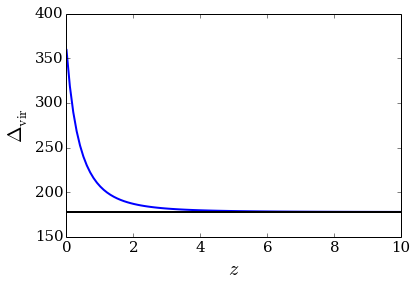
\includegraphics[scale=0.5]{../figures/deltavir.png}
\caption{The solid blue line shows the behaviour of $\Delta_{vir}$
as function of the redshift. The black line show the value of
$\Delta_{vir}=173$ at $z>4$}
\end{figure}

The virial density now can be expressed in terms of $\Delta_{vir}$:

\begin{equation}\label{eq:rhovir}
\rho_{vir} = \frac{3M_{vir}}{4 \pi r_{vir}^3} = \Delta_{vir} \Omega_m \rho_{crit} 
\end{equation}

Where $\Omega_m$ is the density parameter that give as the abundance of matter in the
Universe, it is define as $\Omega_m = \rho / rho_c$ and the actual value is $\Omega_m \simeq 0.3$
Once the virial density is defined with \ref{eq:rhovir} for a given $z$ then the radius
and the virial mass can be related:

\begin{equation}
r_{vir} = \left( \frac{3M_{vir}}{4 \pi \Delta_{vir} \Omega_m \rho_{crit} } \right )^{1/3}
\end{equation}

For example for a halo of mass $M = 1 \times 10^{12}M_{\odot}$ the corresponding radius
is $r_{vir}=262.4$ Kpc
\subsection{$r_{200}$ \& $M_{200}$}

There is another radious and mass of particular interest. This is the radius that enclosed a density
of 200 times the density of the Universe. $M_{200}$ is defined as:

\begin{equation}\label{eq:m200}
M_{200} = 200 \rho_c \dfrac{4}{3} \pi r_{200}^3
\end{equation}

In the same way $M_{vir}$ is defined as:

\begin{equation}\label{eq:mvir}
M_{vir} = \Delta_{vir} \Omega_m \rho_c \dfrac{4}{3} \pi r_{vir}^3
\end{equation}

The critial density $\rho_c$ is the same for both cases, then it is possible
to relate both masses from Eq\ref{eq:m200} and Eq\ref{eq:mvir} as follows:

\begin{equation}
\dfrac{M_{200}}{M_{vir}} = \left(  \dfrac{200}{ \Delta_{vir} \Omega_m}  \right) \left( \dfrac{r_{200}}{r_{vir}}  \right)^3
\end{equation}

Here is common to call $q = \left(  \dfrac{200}{ \Delta_{vir} \Omega_m}  \right) $,  at $z=0$ $q=2.053$.

\begin{equation}\label{eq:q}
\dfrac{M_{200}}{M_{vir}} = q \left( \dfrac{r_{200}}{r_{vir}}  \right)^3
\end{equation}

This Eq.\ref{eq:q} relates $M_{vir}$ and $M_{200}$ for a given $r{vir}$ and $r_{200}$.

\begin{figure}[H]
\centering
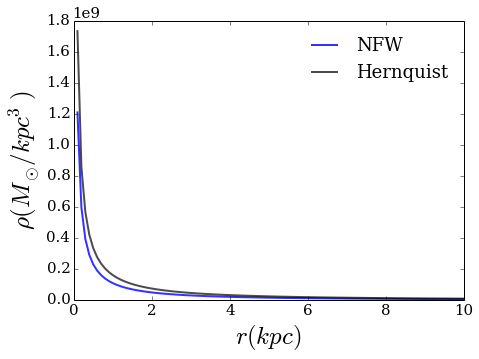
\includegraphics[scale=0.7]{../figures/hernquistNFW.png}
\end{figure}


\chapter{Spherical}
\label{sec:spherical}
\section{Spherical Potentials}

\subsection{Plummer}

The plumer density profile is one of the simplest models which describes
a constant density near the center and falls at large radius.

\begin{equation}
\Phi_P(r) = - \frac{GM}{\sqrt{r^2+a^2}}
\end{equation}


Where $a$ is call the scale length. The scale length set the length $a$ in which the mayority of the density is enclosed. Note
that if $a$ is cero the plummer potential would be exactly as the potential of a point mass.
In the other hand if $a$ goes to infinity the potential is represents a very extended mass source.
In other words the scale length set up the size of the volume in which the mass $M$ is enclosed.

Making use of the Poisson's equation one can derive the density from the potential and vice versa.

\begin{equation}
\nabla ^2 \Phi_P(r) = 4 \pi G \rho_P(r) = \frac{1}{r^2}\frac{d}{dr} \left (  r^2 \frac{d\Phi_P(r)}{dr} \right)
\end{equation}

\begin{equation}
\rho_P (r) = \frac{3M}{4\pi a^3} (1 + \frac{r^2}{a^2})^{-5/2}
\end{equation}


The enclosed mass can be derived from the density by integrating over a volume or radius r.

\begin{equation}
M_P(<r) = 4 \pi \int_0^r r'^2\frac{3M}{4\pi a^3} (1 + \frac{r'^2}{a^2})^{-5/2} dr' = \frac{3M}{a^3} \left( \frac{a^4 r^3 \sqrt{r^2/a^2 + 1}}{3(r^2 + a^2)^2}  \right)
\end{equation}

Making some algebra the total mass enclosed in radius $r$ is 
given by:

\begin{equation}
M_P(<r) = M \frac{r^3}{(a^2+r^2)^{3/2}}
\end{equation}

The cirular velocity can be derived from the total enclosed mass
as follows:

%begin{equation}
%_g = \frac{GmM}{r^2} = ma_c = m \frac{v_c^2}{r}
%end{equation}

\begin{equation}
v_c = \sqrt{\frac{GM(<r)}{r}}
\end{equation}

\begin{equation}
v_c = \sqrt{GM\left(\frac{r^2}{( r^2+a^2 ) ^{3/2}}\right)}
\end{equation}


Finally the acceleration can be derived using:

\begin{equation}
a = - \nabla \Phi 
\end{equation}

\begin{equation}
a = - \dfrac{GMr}{(r^2 + a^2)^{3/2}} 
\end{equation}

All this quantities are plotted in Fig.\ref{fig:plummer}.

\begin{figure}[H]
\centering
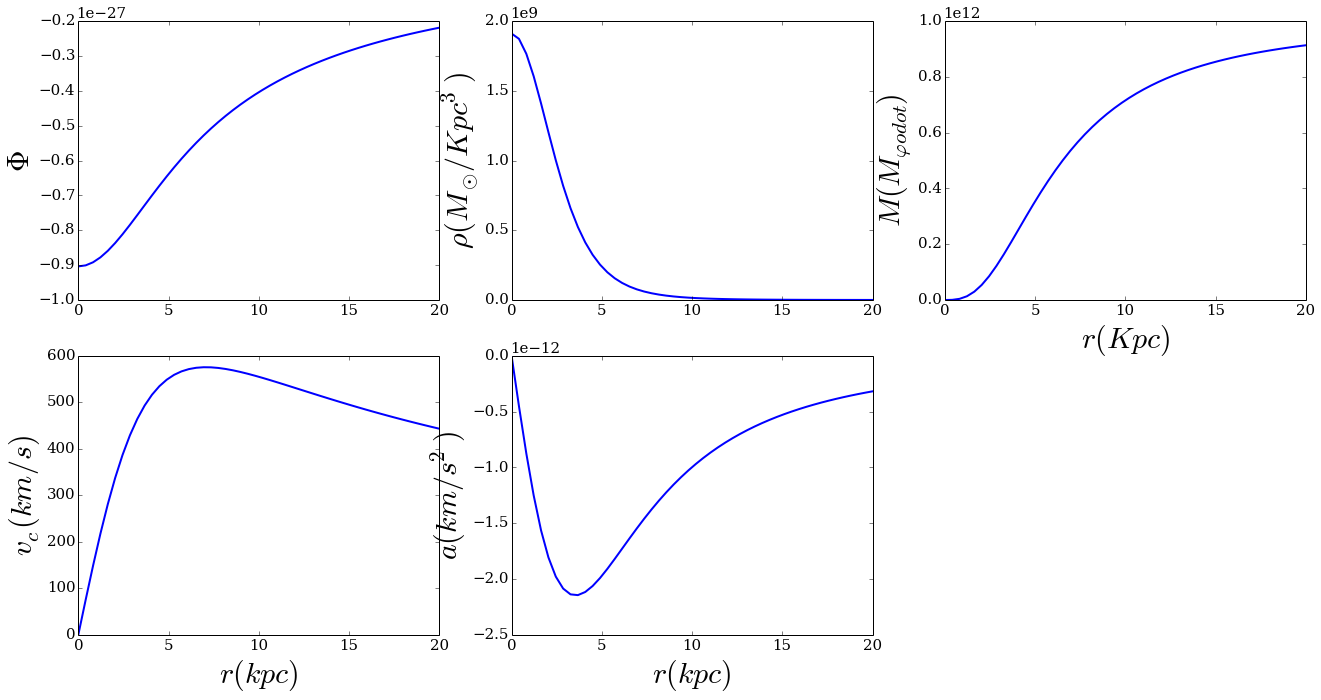
\includegraphics[scale=0.35]{../figures/plummer.png}
\label{fig:plummer}
\end{figure}

\ref{fig:plummer}

\subsection{Hernquist profile}

The Hernquist profile is derived in such a way that it follows the

\begin{equation}
\rho_{Hernquist}(r) =  \frac{M}{2\pi} \frac{a}{r(r+a)^3}
\end{equation}

\begin{equation}
M_{Hernquist}(<r) = 2aM \int \frac{r}{(r+a)^3}dr
\end{equation}

\begin{equation}
M_{Hernquist}(<r) = M \frac{r^2}{(r+a)^2}
\end{equation}

\begin{equation}
\Phi = - \frac{GM}{r+a}
\end{equation}

\begin{equation}
v_c(r) = GM \frac{r}{(r+a)^2}
\end{equation}

\begin{equation}
a = - \dfrac{GM}{(r+a)^2}
\end{equation}


\begin{figure}[H]
\centering
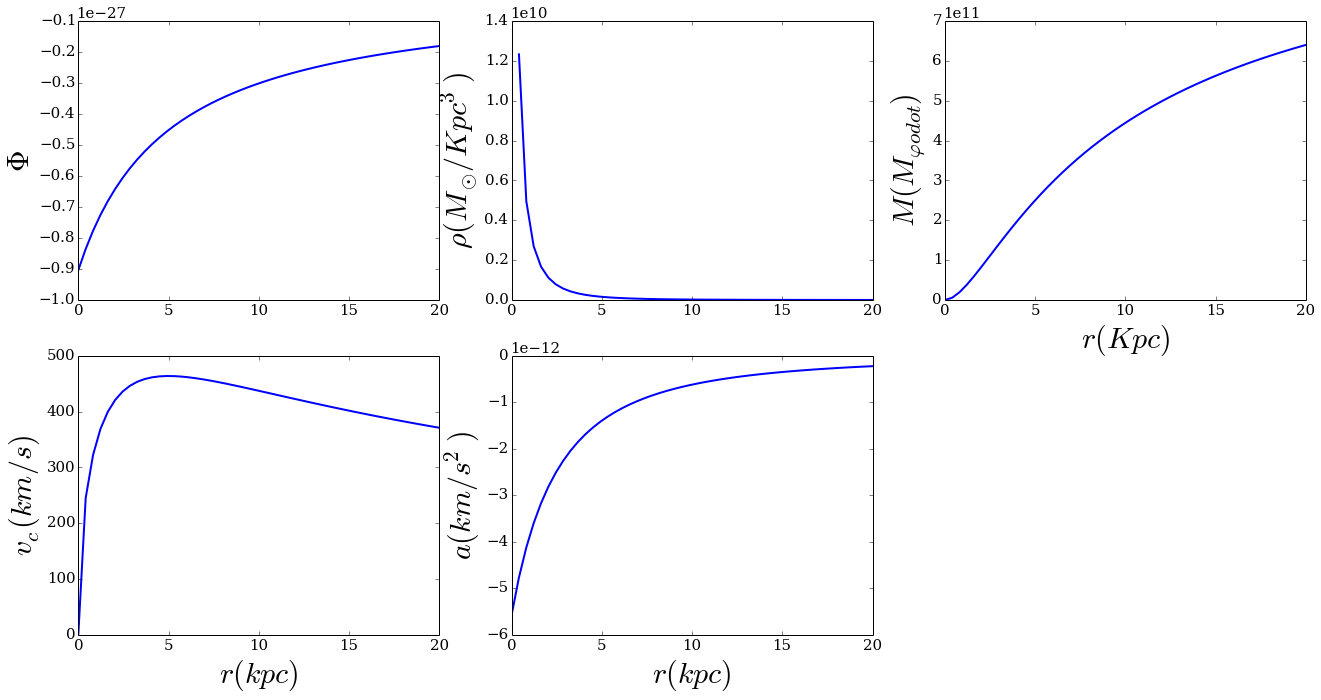
\includegraphics[scale=0.35]{../figures/hernquist.png}
\end{figure}



\subsection{Singular Isothermal Sphere}

The Singular Isothermal Sphere (\textbf{SIS}) describes a system in which the particles follow
a Maxwellian density distribution. With this distribution and the Poisson equation the follow
density profiles could be derived.


\begin{equation}
\rho_{iso}(r) = \dfrac{\sigma ^2}{2\pi G (r^2+a^2)}
\end{equation}

Following the same procedure as with the previuos profiles we find $M, \Phi$  and $v_c$.

\begin{equation}
M_{iso}(<r) = \dfrac{2 \sigma (r+a)}{G}
\end{equation}

\begin{equation}
\Phi_{iso}(r) = 2 \sigma^2 ln(r+a)  + const.
\end{equation}

\begin{equation}\label{eq:SISv}
v_c(r) = \sqrt{2}\sigma
\end{equation}

\begin{equation}
a = - \dfrac{v^2}{(r+a)}
\end{equation}

This profile is quite different to the previous ones due to the fact that here the input is
the velocity instead of the total Mass.

\begin{figure}[H]
\centering
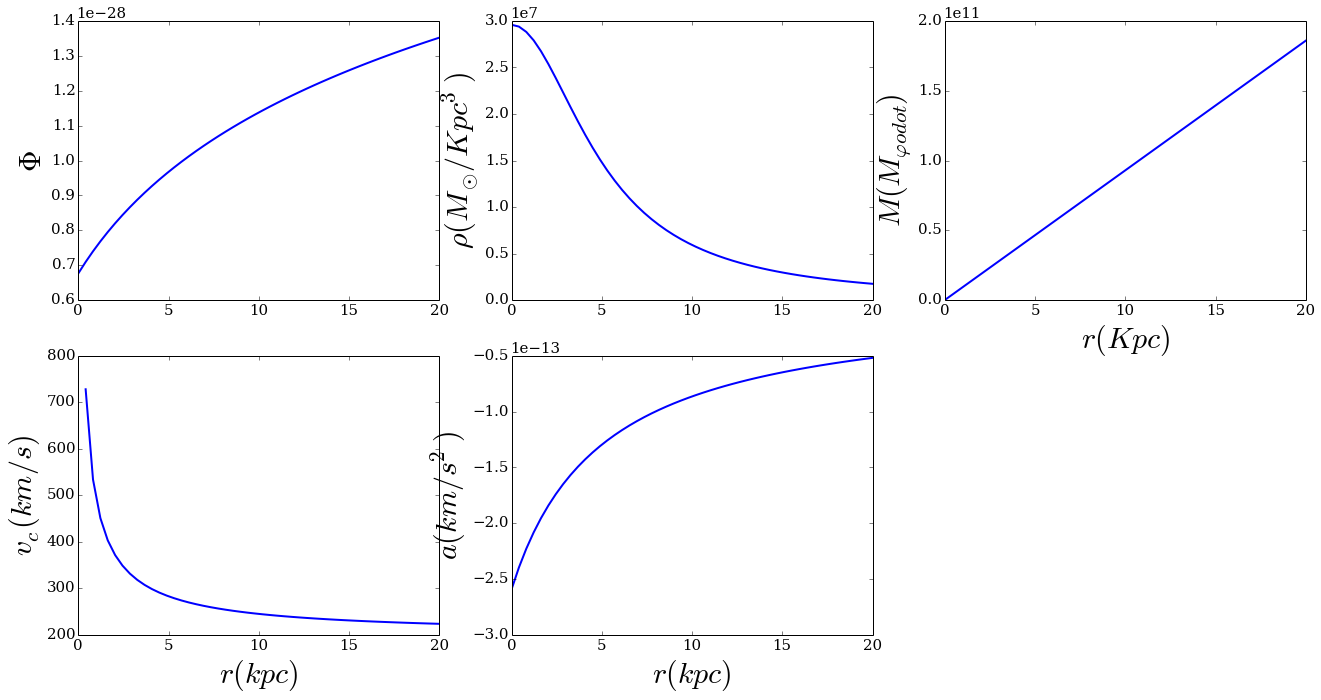
\includegraphics[scale=0.35]{../figures/sis.png}
\end{figure}




\subsection{NFW}


\begin{equation}\label{eq:rhoNFW}
\rho_{NFW}(r) = \dfrac{\rho_s}{(r/a) (1 + r/a)^2}
\end{equation}


\begin{equation}\label{eq:MNFW}
M_{NFW}(r) =  M  \left(  ln(1 + x) - \frac{x}{1 + x} \right)
\end{equation}

Where $x = r/a$, is useful to define the function $f(x)$ as:

\begin{equation}
f(x) = ln(1 + x) - \frac{x}{1 + x} 
\end{equation}

Then \ref{eq:MNFW} can be expresed as:

\begin{equation}\label{eq:M2NFW}
M_{NFW} = 4 \pi \rho_s a^3 f(x) = M_{vir}f(x)/f(c_{vir})
\end{equation}

\begin{equation}\label{PhiNFW}
\Phi_{NFW} = -4\pi G M \frac{ln(1 + r/a)}{r}
\end{equation}

\begin{equation}\label{eq:cnfwz0}
c(M_{vir}) = 9.60  \left( \frac{M_{vir}}{10^{12}h^{-1}M_{\odot}} \right)^{-0.075}
\end{equation}



\begin{equation}\label{vcNFW}
v_c(r) = \sqrt{\left(\dfrac{M(r)G}{r}\right)} = \sqrt{\left( \dfrac{2 M  \left(  ln(1 + c) - \frac{c}{1 + c} \right)}{r} \right)}
\end{equation}


\begin{figure}[H]
\centering
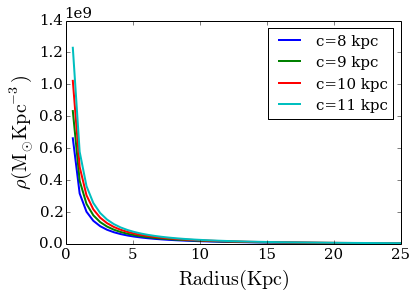
\includegraphics[scale=0.7]{../figures/NFW_density.png}
\end{figure}

\begin{figure}[H]
\centering
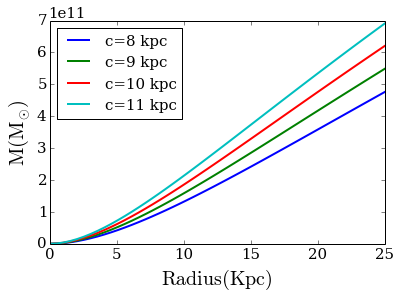
\includegraphics[scale=0.7]{../figures/NFW_mass.png}
\end{figure}

\begin{figure}[H]
\centering
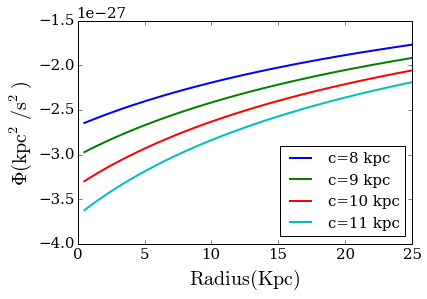
\includegraphics[scale=0.7]{../figures/NFW_potential.png}
\end{figure}

\begin{figure}[H]
\centering
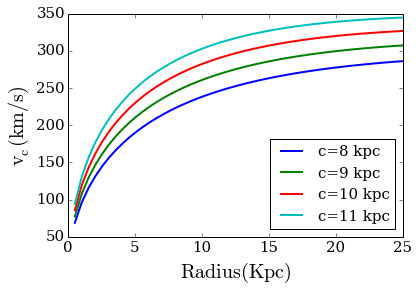
\includegraphics[scale=0.7]{../figures/NFW_vc.png}
\end{figure}



\section{Conversion from NFW to the Hernquist profile}

The average density of the NFW distribution can be expressed as:

\begin{equation}
\bar \rho_{NFW}(r) = \dfrac{3M_{NFW}(r)}{4 \pi r^3} 
\end{equation}

And with eq.\ref{eq:M2NFW} the $\bar{\rho_{NFW}(r)}$ takes de form:

\begin{equation}
\bar \rho_{NFW}(r) = 3 \rho_a \left( \dfrac{a}{r} \right)^{3}  f(x)
\end{equation}

Now if we want to find the relationship betwee $r_{200}$ and $r_{vir}$
for the NFW profile we have to apply eq\ref{eq:q}.

\begin{equation}
q = \dfrac{3 \rho_a \dfrac{a}{r_{200}} f(c_{200})}{3 \rho_a \dfrac{a}{r_{vir}}f(c)} = \dfrac{c_{200}^{3}f(c_{200})}{c_{vir^3}f(c_{vir})}
\end{equation}


\begin{equation}\label{eq:c200cvir}
\dfrac{c_{200}}{c_{vir}} = \left( \dfrac{f(c_{200})}{qf(c_{vir})} \right)^{1/3}
\end{equation}

For $c_{vir} = 10$ this function is shown in Fig.\ref{fig:c200cvir}, where
$y = \dfrac{c_{200}}{c_{vir}} - \left( \dfrac{f(c_{200})}{qf(c_{vir})} \right)^{1/3}$

\begin{figure}[H]\label{fig:c200cvir}
\centering
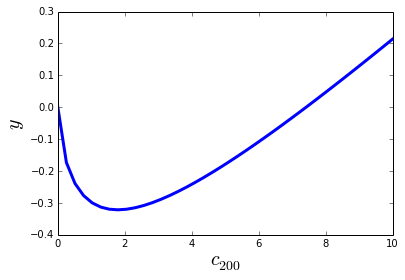
\includegraphics[scale=0.7]{../figures/c200cvir.png}
\end{figure}

Note that the solution of Eq.\ref{eq:c200cvir} is when $y=0$, one
solution is $c_{200}=0$ but this is not of particular interest for us.

The other solution is computed analytically using the bisection algorithm.
$c_{200} = 7.4$

In order to seek the equivalence between the NFW and the Hernquist profile,
We have to match the same enclosed mass of both profiles at a given radius.
To his end we have to find $M_H$ in terms of $r_s$.

\begin{equation}
M_H(r) = M_{NFW}(r)
\end{equation}

\begin{equation}
\frac{M_H r^2}{a^2 + r^2} = 4 \pi \rho_s r_s^3 \left[ Ln(1 + x) - \frac{x}{1+x}  \right]
\end{equation}

In the limit $r \rightarrow 0$

\begin{equation}
M_H = \dfrac{4 \pi \rho_s r_s^3 a^2}{r^2} \left[ (x - \dfrac{x^2}{2}) - x  \right]
\end{equation}

\begin{equation}
M_H = 4 \pi \rho_s r_s^3 \dfrac{a^2}{r^2} \left(  - \dfrac{r^2}{2r_s^2} \right)
\end{equation}

\begin{equation}
M_H = 2 \pi r_s a^2
\end{equation}

With this relation is possible now to match both profiles at a given radius $\tilde{r}$

\begin{equation}
M_H(\tilde{r}) = M_{NFW}(\tilde{r}) 
\end{equation}

\begin{equation}
2 \pi \rho_s a^2 r_s \dfrac{\tilde{r}^2}{a^2} \dfrac{1}{\left( 1 + \dfrac{\tilde{r}}{a}\right)^2} = 4 \pi \rho_s r_s^3 \left( Ln \left(1 + \dfrac{\tilde{r}}{r_s} \right)  - \dfrac{\tilde{r}}{\tilde{r} + r_s} \right)
\end{equation}

\begin{equation}
\dfrac{\tilde{r}^2 a^2}{(a + \tilde{r})^2} = 2 r_s^2 \left( Ln \left (1 +  \dfrac{\tilde{r}}{r_s} \right)  - \dfrac{\tilde{r}}{\tilde{r} + r_s}   \right)
\end{equation}


\begin{equation}
\dfrac{\tilde{r}^2 a^2}{(a + \tilde{r})^2} = 2 r_s^2 f(\tilde{x})
\end{equation}

\begin{equation}
\left( \frac{a}{r_s} \right)^2 = \dfrac{2}{\tilde{r}^2} (a + \tilde{r})^2 f(\tilde{x})
\end{equation}




\begin{equation}
\dfrac{a}{r_s} = \dfrac{[2 f(\tilde{x})]^{1/2}}{\tilde{r}} (a + \tilde{r})
\end{equation}

\begin{equation}
\left( \dfrac{a}{r_s} \right) \left( 1 -  \dfrac{[2 f(\tilde{x})]^{1/2}}{\tilde{x}} \right) = [2 f(\tilde{x})]^{1/2} 
\end{equation}

\begin{equation}
\dfrac{a}{r_s} = \dfrac{[2 f(\tilde{x})]^{1/2}}{ \left( 1 -  \dfrac{[2 f(\tilde{x})]^{1/2}}{\tilde{x}} \right)}
\end{equation}

\begin{equation}
\dfrac{a}{r_s} = \dfrac{[2 f(\tilde{x})]^{1/2} \tilde{x}}{\tilde{x} - (2f(\tilde{x})^{1/2})} = \dfrac{1}{\left(  [2 f(\tilde{x})]^{-1/2} - \dfrac{1}{\tilde{x}}  \right)}
\end{equation}

Finally the ratio of the enclosed mass of the Hernquist and the NFW profiles is:

\begin{equation}
\dfrac{M_H}{M_{vir}} = \dfrac{2 \pi \rho_s a^2 r_s}{4 \pi \rho_s r_s^3 f(c_{vir})} = \dfrac{1}{2 f(c_{vir})}  \left( \dfrac{a}{r_s}\right)^2
\end{equation}




\chapter{Discs}\label{sec:Discs}
\section{Disc Potentials}

\subsection{Miyamoto-Nagai potential}

For describing discs potentials it is better to change to 
cylindrical coordinates (R, z, $\phi$). The most known and 
used profile is the Miyamoto-Nagai profile \citep{Miyamoto75}. 

\begin{equation}
\Phi_M (R, z) = - \dfrac{GM}{\sqrt{R^2 + (a + \sqrt{(z^2 + b^2)})^2}}
\end{equation}

\begin{equation}
\rho_M (R, Z) = \left( \dfrac{b^2 M}{4 \pi} \right) \dfrac{aR^2 + (a + 3\sqrt{z^2+b^2})(a + \sqrt{z^2+b^2})^2}{[R^2 + (a^2 + \sqrt{z^2+b^2})^2]^{5/2}(z^2+b^2)^{3/2} }
\end{equation}


\begin{equation}
v_c = \sqrt{\dfrac{GMR}{(R^2 + (a + \sqrt{z^2 + b^2})^2)^{3/2}}}
\end{equation}

\begin{equation}
M(r) = \dfrac{v_c^2 r}{G} 
\end{equation}

\begin{equation}
M(<r) = \dfrac{M R^3}{(R^2 + (a + \sqrt{z^2+b^2})^2)^{3/2}}
\end{equation}

\begin{equation}
\vec{a} = \dfrac{-GMR}{(R^2 + (a + \sqrt{z^2 + b^2})^2)^{3/2}} \mathbf{\hat{R}} - \dfrac{GMz (a + \sqrt{z^2+b^2})}{(R^2 + (a + \sqrt{z^2 + b^2})^2)^{3/2}\sqrt{z^2+b^2}} \mathbf{\hat{z}}
\end{equation}

\begin{figure}[H]\label{fig:MN}
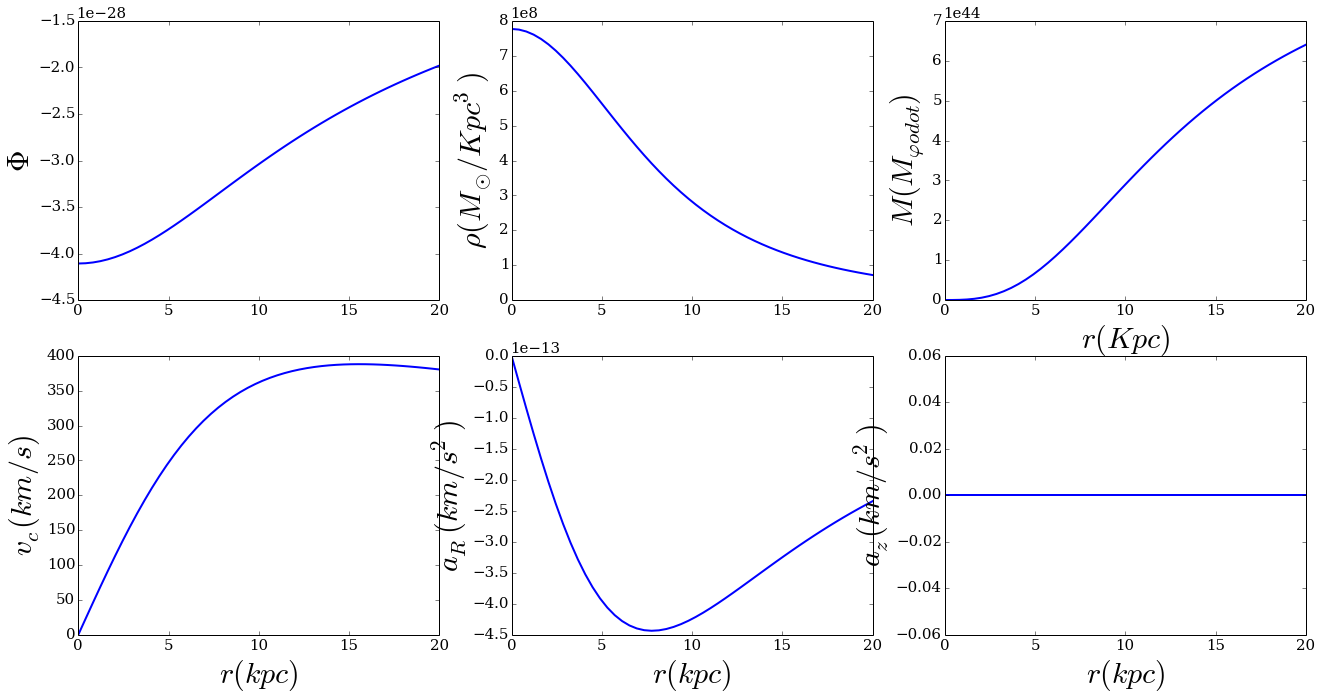
\includegraphics[scale=0.35]{../figures/mn.png}
\end{figure}

\begin{figure}[H]\label{fig:MN_density}
\centering
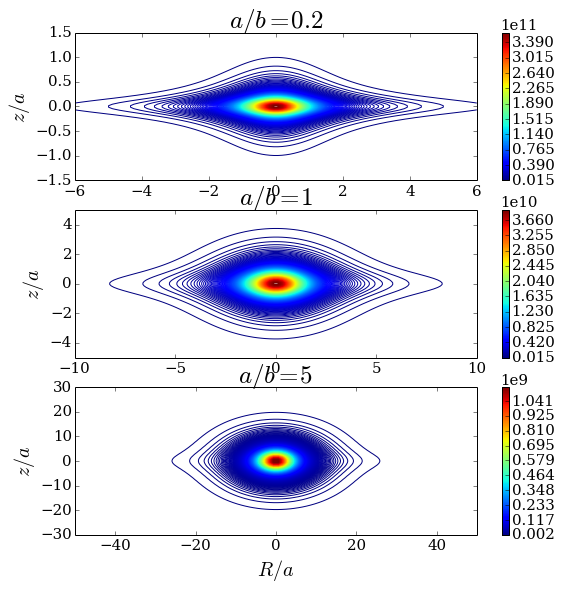
\includegraphics[scale=0.7]{../figures/MN_density_contours.png}
\end{figure}

\section{Logarithmic Profile}\label{sec:log}

\begin{equation}
\Phi_L(R, z) = \dfrac{1}{2} v_0^2 ln \left( R_c^2 + R^2 + \dfrac{z^2}{q_{\phi}^2}  \right) + constant
\end{equation}

The circular velocity is $v_c^2(R, z) = R \dfrac{d \Phi}{dR}$:

\begin{equation}
v_c(R, z=0) =\sqrt{ R \dfrac{d \Phi_L}{dr}} = \dfrac{v_0 R}{\sqrt{R_c^2 + R^2 + z^2/q_{\phi}^2}}
\end{equation}



\begin{figure}[H]
\centering
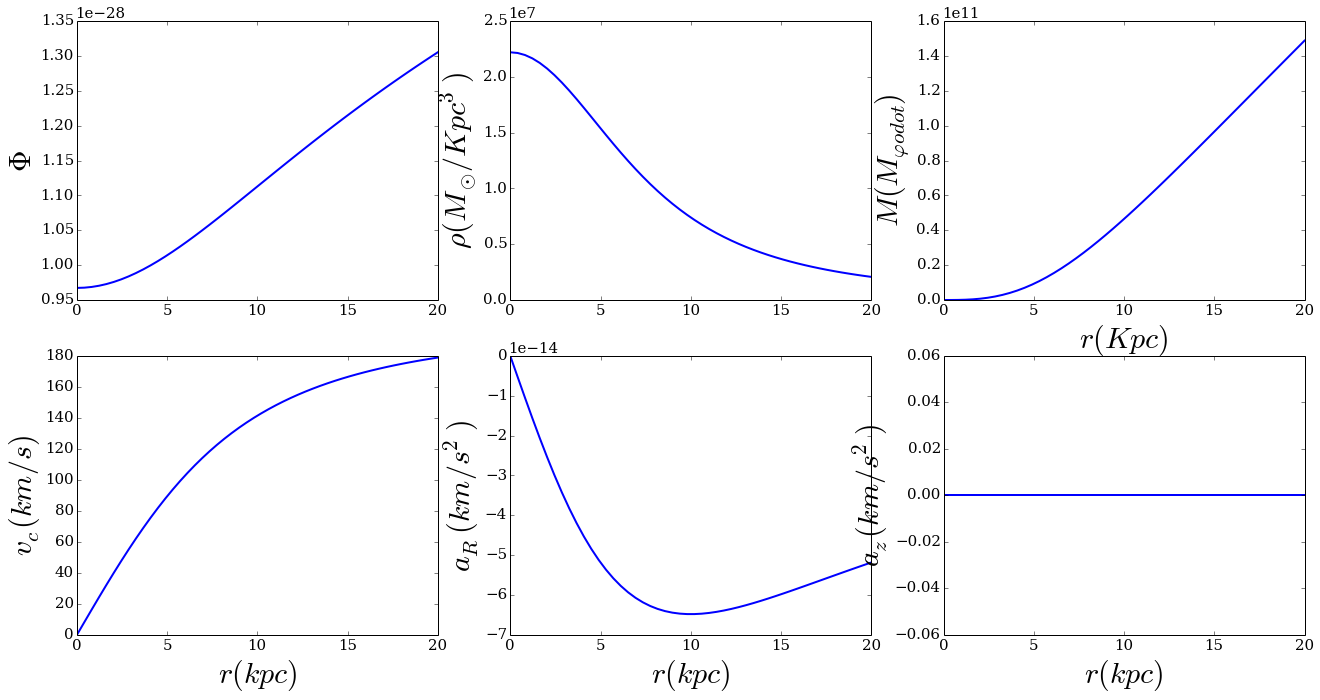
\includegraphics[scale=0.35]{../figures/logarithmic.png}
\end{figure}

\begin{equation}
M(<R) = \dfrac{v_0^2 R^3}{G (R_c^2 + R^2 + z^2/q_{\phi}^2)} 
\end{equation}


To derive the density we make use of Poisson's equation in cylindrical coordinates:

\begin{equation}
\rho_L(R, z) = \dfrac{\nabla^2 \Phi_L}{4 \pi G } = \dfrac{1}{4 \pi G} \left( \dfrac{1}{r}\dfrac{d}{dR}R\dfrac{d}{dR}  + \dfrac{d^2}{dz^2}  \right) \Phi_L
\end{equation}

\begin{equation}
\rho_L(R, z) = \dfrac{v_0^2}{8 \pi G } \left( \dfrac{1}{R} \dfrac{4R ( R_c^2 + R^2 + \dfrac{z^2}{q_{\phi}^2} ) - 4R^3}{( R_c^2 + R^2 + \dfrac{z^2}{q_{\phi}^2} )^2} + \dfrac{\dfrac{2}{q_{\phi}^2} ( R_c^2 + R^2 + \dfrac{z^2}{q_{\phi}^2} ) - \dfrac{4z^2}{q_{\phi}^4}}{( R_c^2 + R^2 + \dfrac{z^2}{q_{\phi}^2} )^2}  \right)
\end{equation}

\begin{equation}
\rho_L(R, z) =  \dfrac{v_0^2}{4 \pi G q_{\phi}^2} \dfrac{(2q_{\phi}^2 + 1)R_c^2 + r^2 + (2 - q_{\Phi^2})z^2}{(R_c^2 + r^2 + z^2q_{\Phi}^{-2})^2}
\end{equation}


\begin{equation}
a =  - \dfrac{v_0^2}{(R_c^2 + R^2 + z^2/q_{\phi}^2)} (R \mathbf{\hat{R}} + z/q_{\phi}^2 \mathbf{\hat{z}}) 
\end{equation}

\begin{figure}[H]
\centering
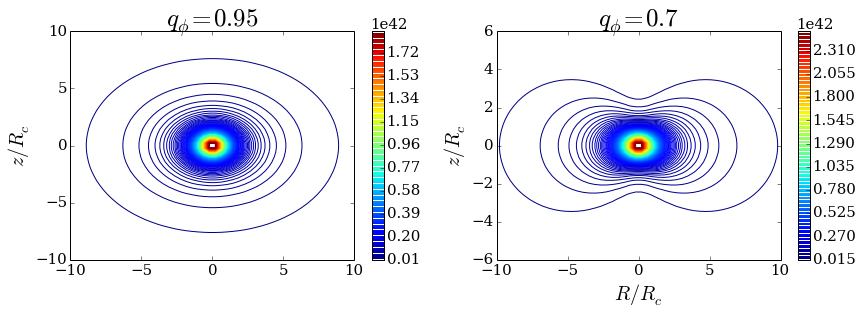
\includegraphics[scale=0.6]{../figures/MN_logarithmic_contours.png}
\end{figure}



\chapter{Triaxial}
\label{sec:Triaxial}
\section{Triaxial Potentials}


\subsection{Logarithmic Triaxial Density Profile}\label{sec:LM10}

Motivated by the fact that the models of the Milky Way Dark Matter halo
at that time can not reproduce the Sgr stream. Mainly because in axisietric
potentials it is not possible to fit the angular precession and the the
distance of the stream. \cite{Law09} propose a triaxial halo Eq.\ref{eq:LMpotential}
which is also in agreement with the CDM paradigm that predicts triaxial halos
rather than  spherical \cite{Lee03}. \cite{Law09} report results of the orbital
integration in which they find that the best fit in their triaxial halo is for $q_z = 1.25$,
 $q_1 = 1.5$ and $\phi=90$. \cite{Law10} made N-body simulations in which they
include the triaxial halo potential.

\begin{equation}\label{eq:LMpotential}
\Phi = v^2_{halo} ln(C_1 x^2 + C_2y^2 + C_3 xy + (z/q_z)^2+ r_{halo}^2)
\end{equation}

Where the constants $C_1, C_2, C_3$ are defined as:
%$R, r$ (Cylindrical, spherical)

\begin{equation}
C_1 = \left( \dfrac{cos^2 \phi}{q_1^2} + \dfrac{sin^2 \phi}{q_2^2}   \right)
\end{equation}

\begin{equation}
C_2 = \left( \dfrac{cos^2 \phi}{q_2^2} + \dfrac{sin^2 \phi}{q_1^2} \right)
\end{equation}

\begin{equation}
C_3 = 2 sin \phi cos\phi \left( \dfrac{1}{q_1^2} - \dfrac{1}{q_2^2} \right)
\end{equation}

\begin{figure}\label{fig:Logarithmic}
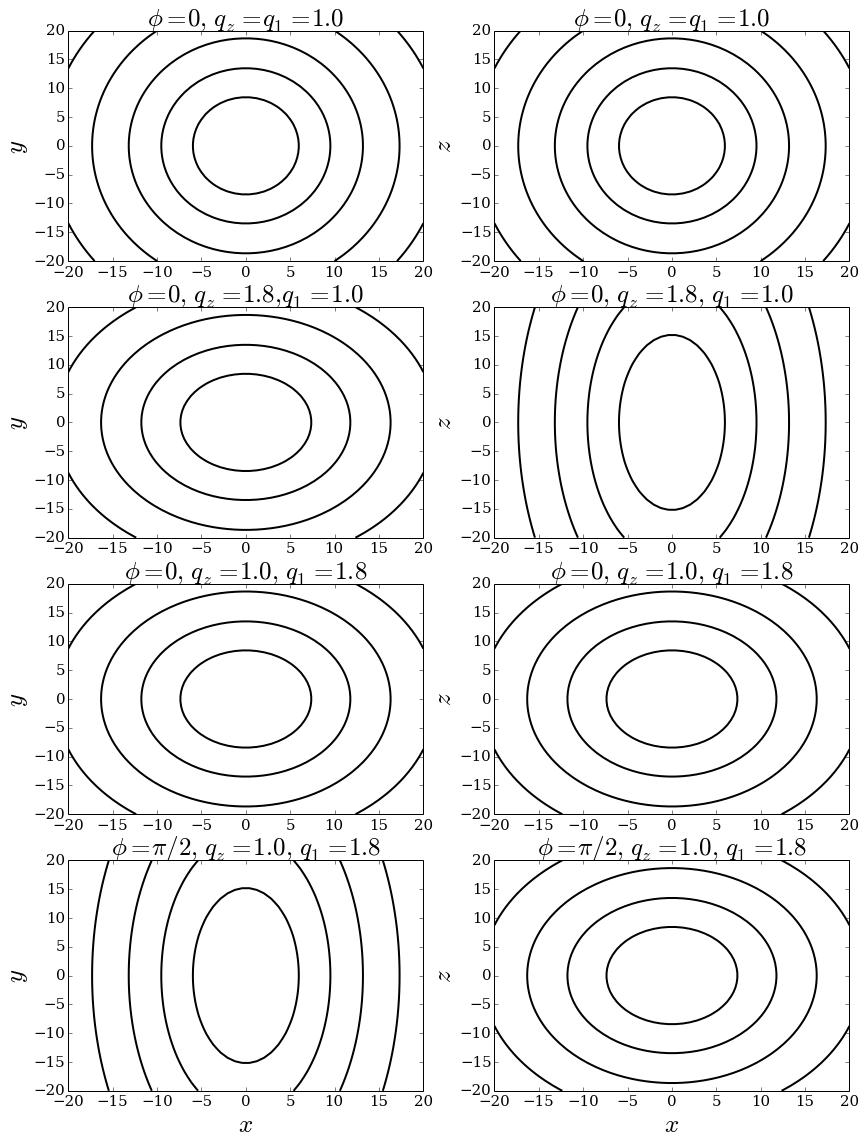
\includegraphics[scale=0.5]{../figures/triaxial_potential.png}
\caption{Logarithmic Triaxial Potential. In the top panel}
\end{figure}



From Eq.\ref{eq:LMpotential} we can derive the circular velocity $v_c$.

\begin{equation}
v_c^2 = r \nabla  \Phi 
\end{equation}

\begin{equation}
\nabla \Phi = \dfrac{d}{dx} \Phi \hat{i} + \dfrac{d}{dy} \Phi \hat{j} + \dfrac{d}{dz} \Phi \hat{k}
\end{equation}

\begin{equation}
\nabla \phi = v_{halo}^2  \left( \dfrac{(2C_1x + C_3 y)\hat{i} + (2C_2y + C_3x)\hat{j} + (2z/q_z^2)\hat{k}}{(C_1 x^2 + C_2 y^2 + C_3 x y + (z/q_z)^2 + r_{halo}^2)}    \right)
\end{equation}

\begin{equation}
v_c = v_{halo} \sqrt{ \dfrac{r((2C_1x + C_3 y)^2 + (2C_2y + C_3x)^2 + (2z/q_z^2)^2)^{1/2}}{(C_1 x^2 + C_2 y^2 + C_3 x y + (z/q_z)^2 + r_{halo}^2)} }
\end{equation}

\citep{LM10} fixed the value of $v_{halo}$ in order that the MW rotation curve reproduce the obervsed value of $v_{LSR}= 220 km/s$ at $R_{\odot}$
this implies that $v_{halo} = 135 km/s$. The rotation curve of is presented in Fig.\ref{vcLM10}, the MW rotation curve is also presented in
Fig.\ref{MWML10} all the paremeters of this rotation curve are summarized in Table\ref{tab:models}.

\begin{figure}[H]\label{fig:vcLM10}
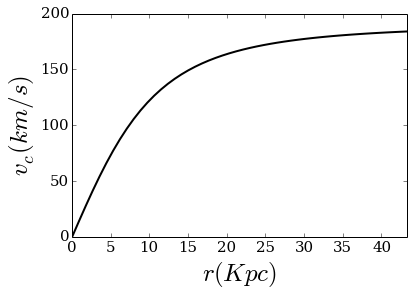
\includegraphics[scale=0.7]{../figures/vcLM10.png}
\end{figure}



\section{Modelling the MW}
\begin{table}[H]\label{tab:models}
%\begin{center}
\begin{scriptsize}
\begin{tabular}{c c c c c }
\hline
Component  &  Besla07 &  LM2010 & Roeland12 & Vera-Helmi13 \\
\hline
Disk Model & Miyamoto-Nagai   & Miyamoto-Nagai &  & Miyamoto-Nagai \\
Disk Mass($M_{\odot}$) & $5.5^{10}$  & $1.0 \times 10^{11}$ & &  $1.0 \times 10^{11}$ \\
Disk Param & $R_d = 3.5$, $z=r_{disk}/5.0$  & $\alpha=1$, $a=6.5 kpc$, $b=0.6 kpc$ & &, $a=6.5kpc$, $b=0.26Kpc$\\
Bulge Model & Hernquist & Hernquist &  & Hernquist\\
Bulge Mass($M_{\odot}$) & $10^{10}$  &$3.4 \times 10^{10}$ & & $3.4\times 10^{11}$\\
Bulge Param & $0.6 kpc$ &  $c=0.7kpc$  & $0.6Kpc$ & $0.7 Kpc$\\
DM halo Model & NFW  & Triaxial \ref{sec:LM10}  & Hernquist(NFW) & Triaxial-Oblate\\
DM halo mass($M_{\odot}$) & $10^{12}$ &$ \times 1.5 \times 10^{12}$ & $10^12$ &\\
Solar Velocity &    &    & 239  & 225.2\\
Halo Param & $c=11, r_{vir} = 258Kpc$ & $r_{halo} = 12 Kpc$ & & $d=12kpc, q_z=0.9, q_1=1.38$\\
 & & & &  $q_2=1, q_3=1.36, \phi=97, r_a=30 kpc$ \\
Solar distance $R_{\odot}$ (kpc) & 8.0 & 8.0  & & 8.0\\
reference &\href{http://adsabs.harvard.edu/abs/2007ApJ...668..949B}{Besla07} & \href{http://bit.ly/1fXtla9}{LM2010} & & \href{http://adsabs.harvard.edu/abs/2013ApJ...773L...4V}{Vera13} \\
\hline
\end{tabular}
\end{scriptsize}
%\end{center}
\end{table}




\begin{figure}[H]\label{MWBesla07}
\centering
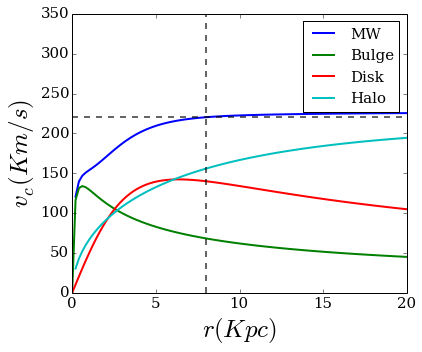
\includegraphics[scale=0.7]{../figures/MWBEsla07.png}
\end{figure}



\begin{figure}[H]\label{MWLM10}
\centering
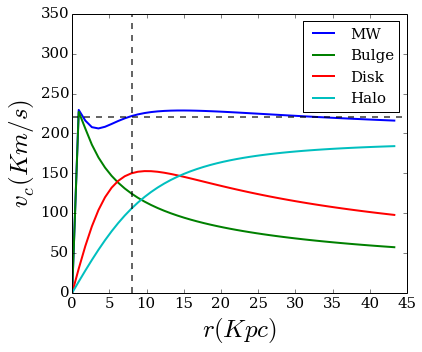
\includegraphics[scale=0.7]{../figures/MWLM10.png}
\end{figure}

\subsection{Vera-Ciro \& Helmi models}

\begin{equation}
\Phi_s(r) = v_{halo}^2 ln(\tilde{r}^2 + d^2)
\end{equation}

\begin{equation}
\tilde{r} = \dfrac{r_a + t_T}{r_a + r_A}r_A
\end{equation}

\begin{equation}
r_A^2 = x^2 + y^2 + \dfrac{z^2}{{q_z}^2} 
\end{equation}

\begin{equation}
r_T ^ 2 = C_1 x^2 + C_2 y^2 + C_3 xy + \dfrac{z^2}{q_3^2}
\end{equation}

Where $C_1, C_2, C_3$ are the same as in the triaxial model. 

\subsubsection{Acceleration}

Then the acceleration would be:

\begin{equation}
a = -\nabla \Phi 
\end{equation}

\begin{equation}
-\nabla \Phi = -v_{halo}^2 \dfrac{2 \tilde{r} }{ (\tilde{r}^2 + d^2)} \left(  \dfrac{d\tilde{r}}{dx} \hat{i} + \dfrac{d\tilde{r}}{dy} \hat{j} + \dfrac{d\tilde{r}}{dz} \hat{k}    \right)
\end{equation}

To evaluate this derivatives the following expressions are useful:

\begin{equation}
\dfrac{\partial r_T}{\partial x} = \dfrac{C_1x + C_3y/2}{(C_1X^2 + C_2y^2 + C_3xy + z^2/q_3^2)^{1/2}}
\end{equation}

\begin{equation}
\dfrac{\partial r_T}{\partial y} = \dfrac{C_2y + C_3x/2}{(C_1X^2 + C_2y^2 + C_3xy + z^2/q_3^2)^{1/2}}
\end{equation}

\begin{equation}
\dfrac{\partial r_T}{\partial z} = \dfrac{z/q_3^2}{(C_1X^2 + C_2y^2 + C_3xy + z^2/q_3^2)^{1/2}}
\end{equation}

\begin{equation}
\dfrac{\partial r_A}{\partial x} = \dfrac{x}{(x^2 + y^2 + z^2/{q_z}^2)^{1/2}}
\end{equation}

\begin{equation}
\dfrac{\partial r_A}{\partial y} = \dfrac{y}{(x^2 + y^2 + z^2/{q_z}^2)^{1/2}}
\end{equation}

\begin{equation}
\dfrac{\partial r_A}{\partial z} = \dfrac{z/q_z^2}{(x^2 + y^2 + z^2/{q_z}^2)^{1/2}}
\end{equation}

\begin{equation}
\dfrac{\partial \tilde{r}}{\partial \alpha} = \dfrac{\left( \dfrac{dr_T}{d\alpha} r_A + r_T \dfrac{dr_A}{d\alpha}\right) (r_a + r_A) - (r_a + r_T)r_A \dfrac{dr_A}{d\alpha} }{(r_a + r_A)^2}
\end{equation}

Where $\alpha$ stands for the $x, y, z$

With these definitions the acceleration terms are:

\begin{equation}
a_x = - \dfrac{v_{halo}^2 2 \tilde{r}}{(\tilde{r}^2 + d^2)} \dfrac{\partial \tilde{r}}{\partial x}
\end{equation}

\begin{equation}
a_y = - \dfrac{v_{halo}^2 2 \tilde{r}}{(\tilde{r}^2 + d^2)} \dfrac{\partial \tilde{r}}{\partial y}
\end{equation}

\begin{equation}
a_z = - \dfrac{v_{halo}^2 2 \tilde{r}}{(\tilde{r}^2 + d^2)} \dfrac{\partial \tilde{r}}{\partial z}
\end{equation}

\subsubsection{Circular velocity}

\begin{equation}
{v_c}^2 = r|-\nabla \phi|  = - \dfrac{2 \tilde{r}^2 v_{halo}^2}{\tilde{r}^2  + d^2} \left( \left( \dfrac{d\tilde{r} }{dx}\right)^2 + \left( \dfrac{d\tilde{r} }{dy}\right)^2 + \left( \dfrac{d\tilde{r} }{dz}\right)^2  \right)^{1/2} 
\end{equation}






\section{code}

Running GalIC on el Gato:

go to \verb+ICs/GalIC+ then charge \verb+gsl+ and \verb+intel-mpi+ modules
and then run \verb+bsub < galic.sh+

\section{TO-DO:}

\begin{itemize}

\item One big figure per profile
\item Put all the acceleration terms
\item Vera-Ciro model
\item Rotation curves of the MW for all the models
\item NFW HErnquist plot equivalence 
\item note: Klypin relation between $c$ and $M_{vir}$ Doesn't take into 
account adiabatic contraction. 

\item work in the code that integrates the orbits using the accelerations. (Viernes)

\end{itemize}

\bibliographystyle{unsrtnat}
\bibliography{referencesDMMW}


\end{document}
